\documentclass[11pt]{article}
\usepackage{url}
\usepackage{graphicx}

\usepackage{course}
\begin{document}


\ctitle{1}{Decision trees and k-Nearest Neighbors}{
Oct. 25, 2022 at 11:59 pm

}
\author{}
\date{}
\vspace{-1in}
\maketitle
\vspace{-0.75in}
\newcommand \img[1]{\includegraphics[width=0.5\linewidth]{#1}}


\blfootnote{Parts of this assignment are adapted from course material by Andrea Danyluk (Williams), Tom Mitchell, Matt Gormley and Maria-Florina Balcan (CMU), Stuart Russell (UC Berkeley), Carlos Guestrin (UW), Dan Roth (UPenn) and Jessica Wu (Harvey Mudd). }



\ifsoln 
\else
\section*{Submission instructions}
\begin{itemize}
\item 
Submit your solutions electronically on the course Gradescope site as PDF files.
\item Please package your code (.ipynb) for Problem 3 and submit it to BruinLearn.
\item If you plan to typeset your solutions, please use the LaTeX solution template. If you must submit scanned handwritten solutions, please use a black pen on blank white paper and a high-quality scanner app.
\end{itemize}
\fi

\ifnotsolution{\newpage}



\section{Splitting Heuristic for Decision Trees \problemworth{25}}

Recall that the ID3 algorithm iteratively grows a decision tree from the root downwards. On each iteration, the algorithm replaces one leaf node with an internal node that splits the data based on one decision attribute (or feature). In particular, the ID3 algorithm chooses the split that reduces the entropy the most, but there are other choices. For example, since our goal in the end is to have the lowest error, why not instead choose the split that reduces error the most? In this problem, we will explore one reason why reducing entropy is a better criterion.

Consider the following setting. Let us suppose each example is described by 4 boolean features: $X = \langle X_1, \ldots, X_4 \rangle$, where $X_i \in \{0, 1\}$. Furthermore, the target function to be learned is $f : X \rightarrow Y$, where $Y =  X_1 \wedge X_2$. That is, $Y = 1$ if $X_1 = 1$ or $X_2 = 1$ otherwise. Suppose that you have the following training data contains all of $2^4$ possible examples:
\begin{table}[H]
\centering
\begin{tabular}{cccc|c}
$X_1$ & $X_2$ & $X_3$ & $X_4$ & $Y$\\ \hline
0 & 0 & 0 & 0 & 0\\
1 & 0 & 0 & 0 & 0\\
0 & 1 & 0 & 0 & 0\\
1 & 1 & 0 & 0 & 1\\
0 & 0 & 1 & 0 & 0\\
1 & 0 & 1 & 0 & 0\\
0 & 1 & 1 & 0 & 0\\
1 & 1 & 1 & 0 & 1\\
\end{tabular}
\quad \quad \quad \quad
\begin{tabular}{cccc|c}
$X_1$ & $X_2$ & $X_3$ & $X_4$ & $Y$\\ \hline
0 & 0 & 0 & 1 & 0\\
1 & 0 & 0 & 1 & 0\\
0 & 1 & 0 & 1 & 0\\
1 & 1 & 0 & 1 & 1\\
0 & 0 & 1 & 1 & 0\\
1 & 0 & 1 & 1 & 0\\
0 & 1 & 1 & 1 & 0\\
1 & 1 & 1 & 1 & 1\\
\end{tabular}
\end{table}

\begin{enumerate}
\item \itemworth{5} Consider constructing a decision tree with only one leaf (the tree in which root is a leaf node and has no internal node) based on these 4 attributes. What is the best $1$-leaf decision tree and what is its error rate (i.e., number of mistakes / total number of data) on these $2^4$ training examples? 

\solution{
    The best 1-leaf decision tree is just a 0 leaf node, meaning every input will be classified as 0, with a 25\% error rate. 
}

\item \itemworth{5} Follow the previous question. Now, let's consider constructing a decision tree with one split. Is there a split that can reduce the error rate? Please specify the attribute that can reduce the error rate if your answer is yes. Otherwise, please discuss why is not. 

\solution{
    There is no split that will reduce the error rate. The minimum possible error rate with a split will still be 25\%.
}

\item \itemworth{5} What is the entropy of the output label $H(Y)$ (rounding to 2 decimal places).

\solution{
    $$ H(y) = -.25log_2(.25) - .75log_2(.75) = .81 $$
    
}

\item \itemworth{5} What is the information gain if we split the data by the attribute $X_1$ ? (rounding to 2 decimal places)

\solution{
    \begin{gather*}
        S_0 = 0 - log_2(1) = 0 \\
        S_1 = -.5log_2(.5) - .5log_2(.5) = 0 \\
        \\
        \text{Gain}(Y, X_1) = .81 - (0 + 0) = .81
    \end{gather*}
}

\item \itemworth{5} What is the information gain if we split the data by the attribute $X_3$? (rounding to 2 decimal places)

\solution{
    \begin{gather*}
        S_0 = -.25log_2(.25) - .75log_2(.75) = .81 \\
        S_1 = -.25log_2(.25) - .75log_2(.75) = .81 \\
        \\
        \text{Gain}(Y, X_3) = .81 - .5(.81 + .81) = 0
    \end{gather*}
}

\end{enumerate}

\pagebreak

\ifsoln 
\else
\clearpage
\fi

\section{k-Nearest Neighbors and Cross-validation \problemworth{20}}
In the following questions you will consider a $k$-nearest neighbor classifier using the Euclidean distance metric on a binary classification task. We assign the class of the test data point to be the class of the majority of the $k$ nearest neighbors. Note that when the test data point is the same as one of the training data point. That training data point can be consider as the closet neighbor of the test data point. 

\begin{figure}[h]
    \centering
    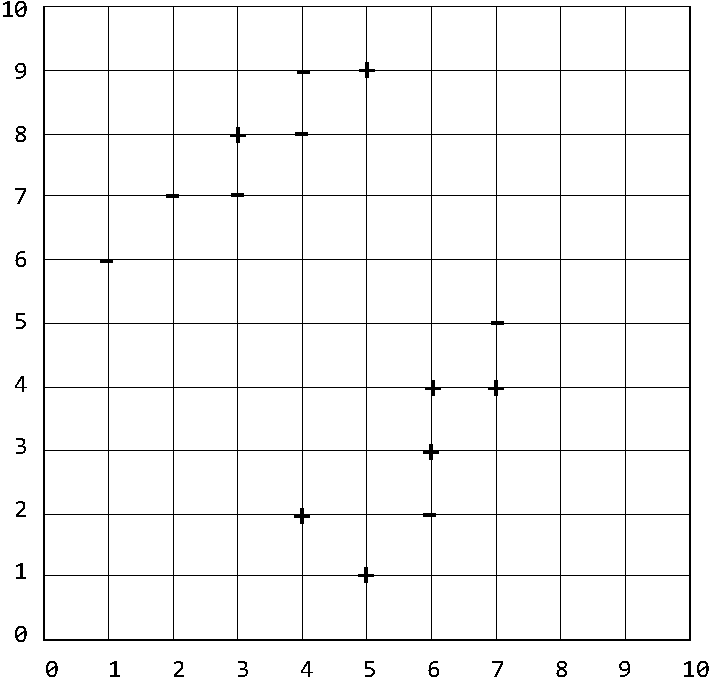
\includegraphics[scale=0.8]{knn_figure.pdf}
    \caption{Dataset for KNN binary classification task.}
    \label{fig:knn}
\end{figure}

\begin{enumerate}
 \item \itemworth{5} 
        What will be the label of point (5,9) in Fig \ref{fig:knn} using k-NN algorithm with majority voting when $k=1$?


    \item \itemworth{5} 
        What will be the label of point (5,9) in Fig \ref{fig:knn} using k-NN algorithm with majority voting when $k=3$?

    \item \itemworth{10}
        Draw the decision boundary of k-NN when $k=1$ on Fig \ref{fig:knn}.

\end{enumerate}
\pagebreak

\newpage
\section{Programming exercise : Applying decision trees and k-nearest neighbors \problemworth{55}}

\section*{Introduction}

\begin{figure}[ht]
\centering
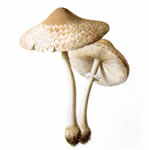
\includegraphics[scale=2.5]{mushroom.jpg}
\end{figure}

In this problem, we will work on a mushroom classification task. The dataset is adapted from the \href{https://archive.ics.uci.edu/ml/datasets/mushroom}{UCI Machine Learning Repository} and it contains descriptions of hypothetical samples corresponding to 23 species of gilled mushrooms. Each mushroom is described in terms of physical characteristics, and the goal is to classify mushrooms as \emph{edible} or \emph{poisonous}. We will apply decision trees and k-nearest neighbors. Since this dataset is relatively simple for classification, we only use 6 features out of 22 features in the original dataset. Features we use include: 
cap-shape, cap-color, gill-color, stalk-root, veil-type, ring-number.


For all the coding, please refer to the following Colab notebook  
\href{https://colab.research.google.com/drive/13_JuaV8-uwTBO7YEheYGm3cjl8DZB8HA?usp=sharing}{Fall2022-CM146-HW1.ipynb}. 

\textbf{Before executing or writing down any code, please make a copy of the notebook and save it to your own google drive by clicking the “File” $\rightarrow$ “Save a copy in Drive”.} 

\begin{figure}[ht]
\centering
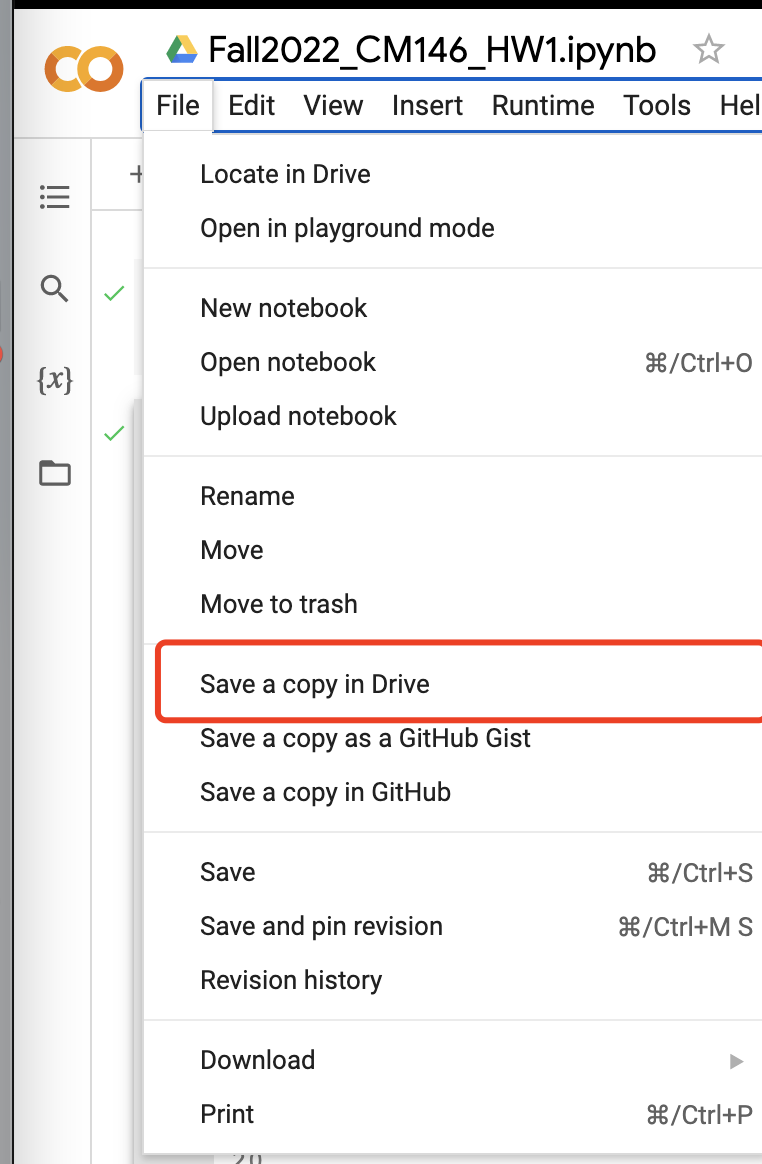
\includegraphics[scale=0.25]{save-colab-to-drive.png}
\end{figure}

You will probably be prompted to log into your Google account. Please make sure all the work you implement is done on your own saved copy. You won’t to able to make changes on the the original notebook shared with the entire class.

The notebook has marked blocks where you need to code:
\begin{verbatim}
### ========== TODO : START ========== ###
### ========== TODO : END ========== ###
\end{verbatim}

\section*{Submission instructions for programming problems}
\begin{itemize}
\item Please save the execution output in your notebook. When submitting, please export the notebook to a \verb|.ipynb| file by clicking ``File'' $\rightarrow$ ``Download .ipynb'' and upload the notebook to BruinLearn.

\item
Your code should be commented appropriately. Importantly:
\begin{itemize}[nosep]
\item Your name should be at the top of the file.
\item Each class and method should have an appropriate doctsring.
\item Include some comments for anything complicated.
\end{itemize}

There are many possible solutions to this assignment, which makes coding style and comments important for graders to conveniently understand the code. 

\item Please submit all the plots and the rest of the solutions (other than codes) to Gradescope.
\end{itemize}


\subsection{Visualizing Features \problemworth{5}}
One of the first things to do before trying any formal machine learning technique is to dive into the data. This can include looking for funny values in the data, looking for outliers, looking at the range of feature values, what features seem important, etc.
We have already included the code for loading the data, converting all the categorical features to numerical one.

Make histograms for each feature, separating the examples by class (i.e., edible or poisonous).
This should produce 6 plots, one for each feature, and each plot should have two overlapping histograms, with the color of the histogram indicating the class. 
The code has been included in \texttt{plot\_histograms} and \texttt{plot\_histogram} functions, and you do not need to code by yourself.

For each feature, what trends do you observe in the data? (Please only describe the general trend. No need for more than two sentences per feature.) 

\solution{
    \begin{itemize}
        \item cap-shape: For both edible and inedible mushrooms the distribution is apprximately symmetrical with edible being slightly skewed left and inedible being slightly skewed right.
        \item cap-color: For both, cap color seems to be evenly spread throughout all possible cap colors. There is no clear trend.
        \item gill-color: For inedible, most gill-color is $<$ 4 while there is no clear trend for edible.
        \item stalk-root: Inedible is largely skewed right while there is no clear trend for edible.
        \item veil-type: There is a clear split between edible and inedible; edible is veil-type $>$ 0 while inedible is veil-type $<$ 0.
        \item ring-number: There is a split between edible and inedible; edible is (mostly) ring-number $>$ 1 while inedible is (mostly) ring-number $<$ 1.
    \end{itemize}
}

\subsection{Training and Evaluating Models \problemworth{55}}

Now, let's use \verb|scikit-learn| to train a \verb|DecisionTreeClassifier| and \verb|KNeighborsClassifier| on the data.
Using the predictive capabilities of the \verb|scikit-learn| package can be carried out in three steps: initializing the model, fitting it to the training data, and predicting new values.

\begin{enumerate}

\item \itemworth{5} Before trying out any classifier, it is often useful to establish a \emph{baseline}. We have implemented one simple baseline classifier, \verb|MajorityVoteClassifier|, that always predicts the majority class from the training set. Read through the \verb|MajorityVoteClassifier| and its usage and make sure you understand how it works.

Your goal is to implement and evaluate another baseline classifier, \verb|RandomClassifier|, that predicts a target class according to the distribution of classes in the training data set. For example, if 85\% of the examples in the training set have \verb|edible = 0| and 15\% have \verb|edible = 1|, then, when applied to a test set, \verb|RandomClassifier| should randomly predict 85\% of the examples as \verb|edible = 0| and 15\% as \verb|edible = 1|.

Implement the missing portions of \verb|RandomClassifier| according to the provided specifications. Then train your \verb|RandomClassifier| on the entire training data set, and evaluate its training error. 

\solution{
    Error: 0.503
}


\item \itemworth{5} Now that we have a baseline, train and evaluate a \verb|DecisionTreeClassifier| (using the class from \verb|scikit-learn| and referring to the documentation as needed). Make sure you initialize your classifier with the appropriate parameters; in particular, use the `entropy' criterion discussed in class. What is the training error of this classifier?

\solution{
    Error: 0.055
}

\item \itemworth{10} Similar to the previous question, train and evaluate a \verb|KNeighborsClassifier| (using the class from \verb|scikit-learn| and referring to the documentation as needed). Use $k$=3, 11 and 19 as the number of neighbors and report the training error of this classifier. If we implement KNN model from scratch, what operations we should do in the \verb|fit| method?

\solution{
    Error (k = 3): 0.064
    Error (k = 11): 0.070
    Error (k = 19): 0.076

    If implemented from scratch, we would need to store the data in our chosen data structure within the fit method. 
}

\item \itemworth{10} So far, we have looked only at training error, but as we learned in class, training error is a poor metric for evaluating classifiers. Let's use cross-validation instead.

Implement the missing portions of \verb|error(...)| according to the provided specifications. You may find it helpful to use \verb|StratifiedShuffleSplit(...)| from \verb|scikit-learn|. To ensure that we always get the same splits across different runs (and thus can compare the classifier results), set the \verb|random_state| parameter to be the same (e.g., 0).


Next, use your \verb|error(...)| function to evaluate the training error and (cross-validation) test error and test micro averaged \href{https://scikit-learn.org/stable/modules/generated/sklearn.metrics.f1_score.html?highlight=f1\%20score#sklearn.metrics.f1_score}{F1 Score} of each of your four models (for the \verb|KNeighborsClassifier|, use $k=11$). To do this, generate a random $85/15$ split of the training data, train each model on the $85\%$ fraction, evaluate the error on both the $85\%$ and the $15\%$ fraction, and repeat this $100$ times to get an average result.


\item \itemworth{10} One way to find out the best value of $k$ for \verb|KNeighborsClassifier| is $n$-fold cross validation.
Find out the best value of $k$ using 5-fold cross validation and the F1 Score metric. Run cross validation for all odd numbers ranging from 1 to 100 as the number of neighbors.

Then plot the validation score against the number of neighbors, $k$. Include this plot in your writeup. What is the best value of $k$ and what is the corresponding score?

You may find the \verb|cross_val_score(...)| from \verb|scikit-learn| helpful. 

\solution{
    The best value of k is 13 with a score of 0.9297682709447415.

    \begin{center}
        \img{./3e.png}
    \end{center}
}


\item \itemworth{10} One problem with decision trees is that they can \emph{overfit} to training data, yielding complex classifiers that do not generalize well to new data. Let's see whether this is the case.

One way to prevent decision trees from overfitting is to limit their depth. Run 20-fold cross-validation for increasing depth limits $1,2,\ldots,20$. 

Then plot the average training F1 Score and test F1 score against the depth limit. Include this plot in your writeup, making sure to label all axes and include a legend for your classifiers. What is the best depth limit to use for this data? Do you see overfitting? Justify your answers using the plot.

You may find \verb|cross_validate| from \verb|scikit-learn| helpful when you want both training scores and validation scores.

\end{enumerate}


\end{document}